
\begin{figure}[ht]
  \centering
  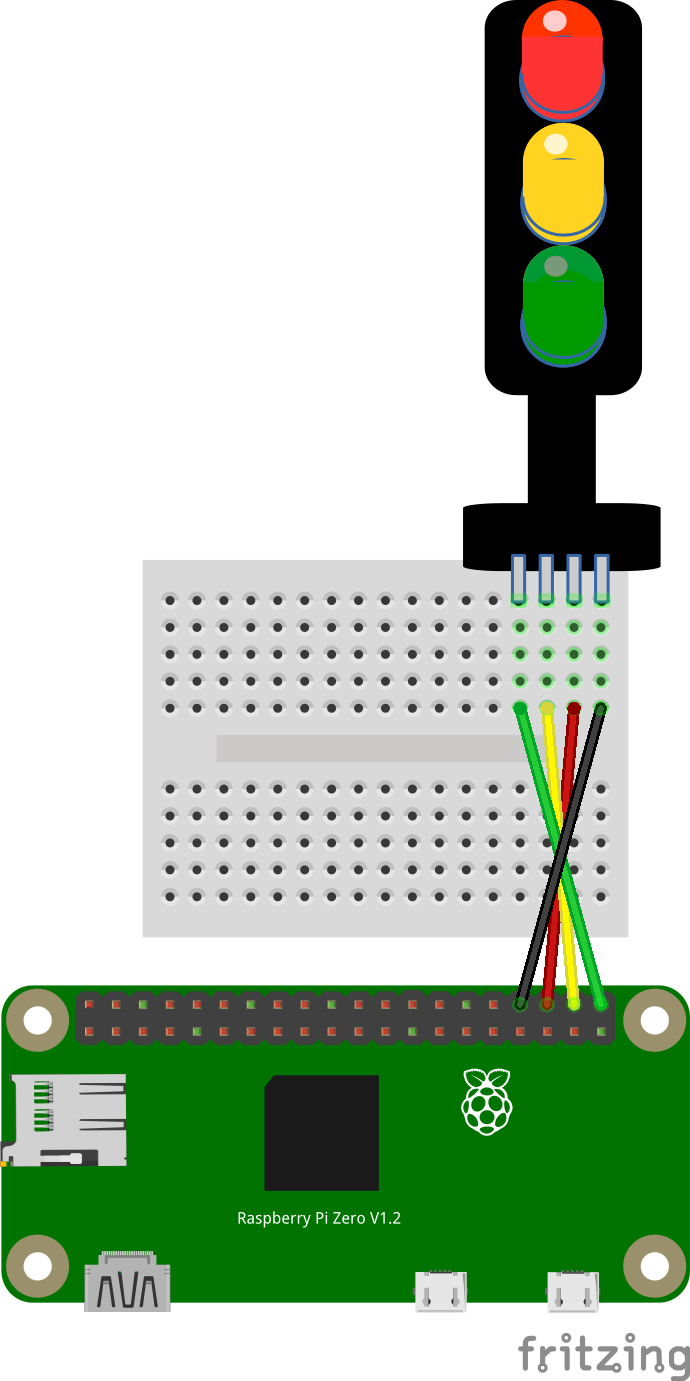
\includegraphics[scale=0.25]{images/TrafficLight_Steckplatine.png}	
  %	\caption{}
  \label{LED_Steckplatine}
\end{figure}

%\begin{figure}[ht]
%	\centering
%	\includegraphics[scale=0.25]{images/TrafficLight_Schaltplan.png}	
%	%	\caption{}
%	\label{LED_Schaltplan}
%\end{figure}

\ExerciseBox{
Bilde die Standardfunktion einer �sterreichischen Ampel nach [Beispiele]\\
Schalte �ber einen Eingang auf Rot f�r den Fu�g�nger�bergang}

%\begin{exercise}
%	Bilde die Standardfunktion einer Ampel nach [Beispiele]\\
%	Schalte �ber einen Eingang sofort auf Rot f�r Fu�g�nger 
%\end{exercise}

\begin{figure}[ht]
	\centering
	
\includegraphics[scale=0.05]{images/Ampel_Rot.png}	
	
\includegraphics[scale=0.05]{images/Ampel_RotGelb.png}
	
\includegraphics[scale=0.05]{images/Ampel_Gruen.png}
	
\includegraphics[scale=0.05]{images/Ampel_Aus.png}
	
\includegraphics[scale=0.05]{images/Ampel_Gruen.png}
	
\includegraphics[scale=0.05]{images/Ampel_Aus.png}
	
\includegraphics[scale=0.05]{images/Ampel_Gruen.png}
	
\includegraphics[scale=0.05]{images/Ampel_Aus.png}
	
\includegraphics[scale=0.05]{images/Ampel_Gruen.png}
	
\includegraphics[scale=0.05]{images/Ampel_Gelb.png}
	%	\caption{}
	\label{Ampel_Ablauf}
\end{figure}

%\subsection{Shell}

\subsection{C}

\begin{console}
	geany &
\end{console}

Nun kann man ein neues Projekt erstellen, dazu w�hlt man \texttt{Projekt} $\rightarrow$ \texttt{Neu...}. Dann Gibt man den Namen des Projekts an. Das Anlegen der Verzeichnisse muss man auch noch best�tigen. 

Danach w�hlt man \texttt{Datei} $\rightarrow$ \texttt{Speichern unter} um die unbenannte Datei mit dem Namen "`TrafficLight.c"' speichern zu k�nnen. Nun kann man den folgenden C-Source eingeben.

\lstset{language=C, caption=, label=TrafficLightProgram, frame=single, basicstyle=\ttfamily
	\footnotesize, breakatwhitespace=false, showstringspaces=false, showtabs=false, tabsize=2 }
\lstinputlisting{source/TrafficLight.c}

Jetzt darf man nicht vergessen im Men� unter \texttt{Erstellen} $\rightarrow$ \texttt{Kommandos zum Erstellen konfigurieren} die Wiring Pi Library mit "`-lwiringPi"' bei Compile und Build zu erg�nzen.

\begin{figure}[ht]
	\centering
	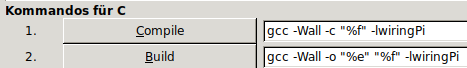
\includegraphics[scale=0.48]{images/Geany_Create_Wiringpi.png}
	%	\caption{}
	\label{Geany-create}
\end{figure}

Nun kann man das Projekt mit den Ziegel-Icon 
\includegraphics[scale=0.4]{images/Geany_Icon_Erstellen.png} erstellen bzw. kompilieren und danach mit dem Zahnrad-Icon 
\includegraphics[scale=0.4]{images/Geany_Icon_Ausfuehren.png}  ausf�hren.  

%\clearpage
\subsection{C\#}

\begin{console}
	geany &
\end{console}

Nun kann man ein neues Projekt erstellen. Dazu w�hlt man \texttt{Projekt} $\rightarrow$ \texttt{Neu...}. Dann gibt man den Namen des Projekts an, z.~B. Raspjamming. Das Anlegen der Verzeichnisse muss danach auch noch best�tigt werden. Nachfolgend unter \texttt{Datei} $\rightarrow$ \texttt{Speichern unter} die unbenannte Datei mit dem Namen "`TrafficLight.cs"' speichern. Nun kann man den folgenden C\#-Source eingeben.\\

\lstset{language=C, caption=, label=TrafficLightProgramCS, frame=single, basicstyle=\ttfamily
	\footnotesize, breakatwhitespace=false, showstringspaces=false, showtabs=false, tabsize=2 }
\lstinputlisting{source/TrafficLight.cs}

Um das Programm kompilieren zu k�nnen, muss im Men� unter \texttt{Erstellen}
$\rightarrow$ \texttt{Kommandos zum Erstellen konfigurieren} der Pfad zur Sourcedatei des C\# WiringPi 
Wrapper (siehe \ref{WiringPiCS}) hinzugef�gt werden. Hierf�r im Textfeld 'Kompilieren' den Pfad z.~B. WiringPi.cs erg�nzen.\\
\texttt{mcs /t:winexe \textquotedblleft\%f\textquotedblright} \textbf{WiringPi.cs} \texttt{/r:System,System.Drawing}\\

\begin{figure}[ht]
	\centering
	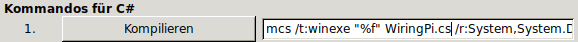
\includegraphics[scale=0.48]{images/Geany_Set_cs.png}
	%	\caption{}
	\label{Geany-setpy3}
\end{figure}

Anschlie�end kann man das Programm mit dem Kompilieren-Icon 
\includegraphics[scale=0.4]{images/Geany_Icon_Kompilieren.png} erstellen bzw. kompilieren und mit dem Zahnrad-Icon 
\includegraphics[scale=0.4]{images/Geany_Icon_Ausfuehren.png} ausf�hren.
Das Programm kann mit der Tastenkombination \framebox{Strg}+\framebox{C} vorzeitig beendet werden.

%\clearpage
\subsection{Python}
Um das Python Programm auszuf�hren muss man eine neue Datei anlegen und 
unter \texttt{Datei} $\rightarrow$ \texttt{Speichern unter} die
Datei mit dem Namen "`TrafficLight.py"' abspeichern. Anschlie�end kann man
folgenden Python-Source einf�gen:

\lstset{language=Python, caption=, 
        label=LEDProgram, frame=single, basicstyle=\ttfamily
	      \footnotesize, breakatwhitespace=false, showstringspaces=false, 
        showtabs=false, tabsize=2 }
\lstinputlisting{source/TrafficLight.py}

Anschlie�end kann man das Programm mit dem Zahnrad-Icon

\includegraphics[scale=0.4]{images/Geany_Icon_Ausfuehren.png}  ausf�hren.  
